\chapter{HR - Employee Attendance and Leave Monitoring}
\minitoc
\clearpage
\section{Introduction}
This chapter presents Sprint 4, focused on HR Employee Attendance and Leave Monitoring, designed to support organization-wide employee visibility, attendance tracking, and leave monitoring. The chapter is organized into three main pages: Employees, Check-In/Out, and Employee Leave.

\section{Sprint Backlog}
The Sprint 4 backlog focused on visibility, traceability, and fast navigation across workforce data.

\begin{table}[H]
\centering
\renewcommand{\arraystretch}{1.2}
\begin{tabular}{|l|>{\raggedright\arraybackslash}p{10.2cm}|l|}
\hline
\textbf{ID} & \textbf{Backlog Item} & \textbf{Priority} \\
\hline
S4-BL-01 & Implement an Employees page with searchable and filterable employee directory data. & High \\
\hline
S4-BL-02 & Add department-based analytics using a donut chart for employee distribution. & Medium \\
\hline
S4-BL-03 & Implement a Check-In/Out page for attendance follow-up with date-based filtering. & High \\
\hline
S4-BL-04 & Implement an Employee Leave page to explain missing check-in/out events. & High \\
\hline
S4-BL-05 & Add cross-page navigation from attendance rows to pre-filtered leave results. & Medium \\
\hline
S4-BL-06 & Ensure pagination and filtering for large datasets using scalable table technologies. & High \\
\hline
\end{tabular}
\caption{Sprint 4 backlog}
\label{tab:sprint-4-backlog}
{\footnotesize\textit{Source: Author's work.}}
\end{table}

\section{Sprint Design}
The design objective was to give HR users a fast workflow from overview to diagnosis: identify employees, inspect attendance events, then check leave reasons when anomalies appear.

\subsection{Employees page design mockup}
The Employees page mockup combines a searchable employee directory with a department-level visualization, helping HR users get a quick organizational overview before deeper attendance analysis.

\begin{figure}[H]
\centering
\IfFileExists{assets/rh/employees-page-design-mockup.jpg}{%
    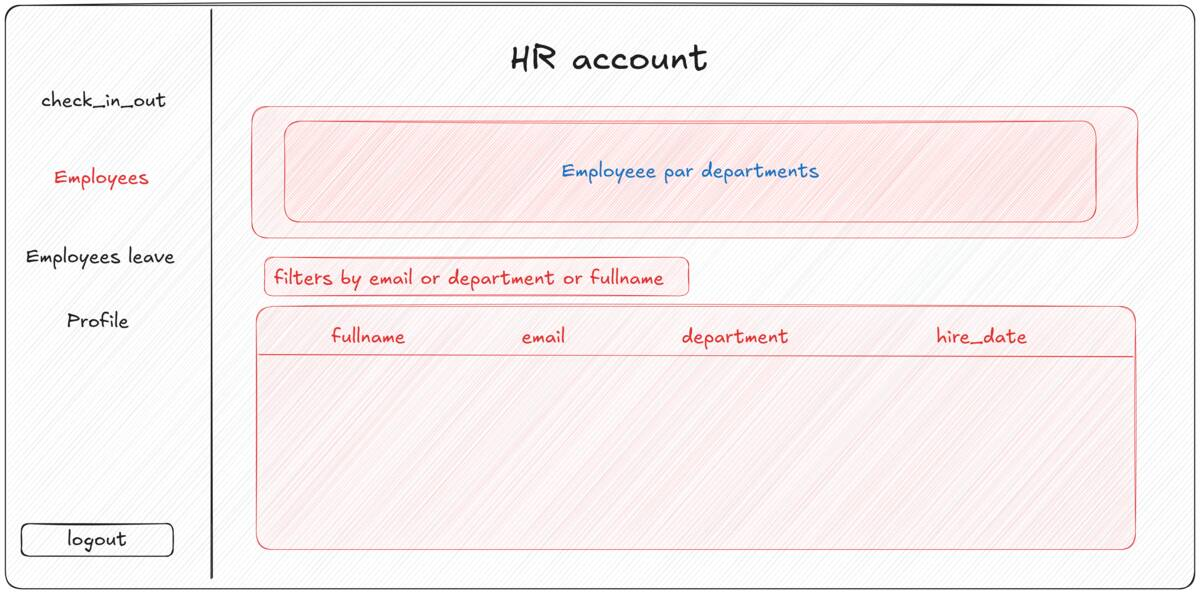
\includegraphics[width=0.92\textwidth,height=0.48\textheight,keepaspectratio]{assets/rh/employees-page-design-mockup.jpg}
}{%
    \fbox{\parbox{0.9\textwidth}{
    \centering
    \vspace{1.6cm}
    \textit{Missing file: assets/rh/employees-page-design-mockup.jpg}\\
    \textit{Insert Employees page design mockup.}
    \vspace{1.6cm}
    }}
}
\caption{Employees Page Design Mockup}
\label{fig:hr-employees-design-mockup}
\end{figure}

\subsection{Check-In/Out page design mockup}
The Check-In/Out page mockup focuses on daily attendance tracking, with clear check-in/check-out records and date-based filters to support operational follow-up by HR users.

\begin{figure}[H]
\centering
\IfFileExists{assets/rh/checkinout-page-design-mockup.jpg}{%
    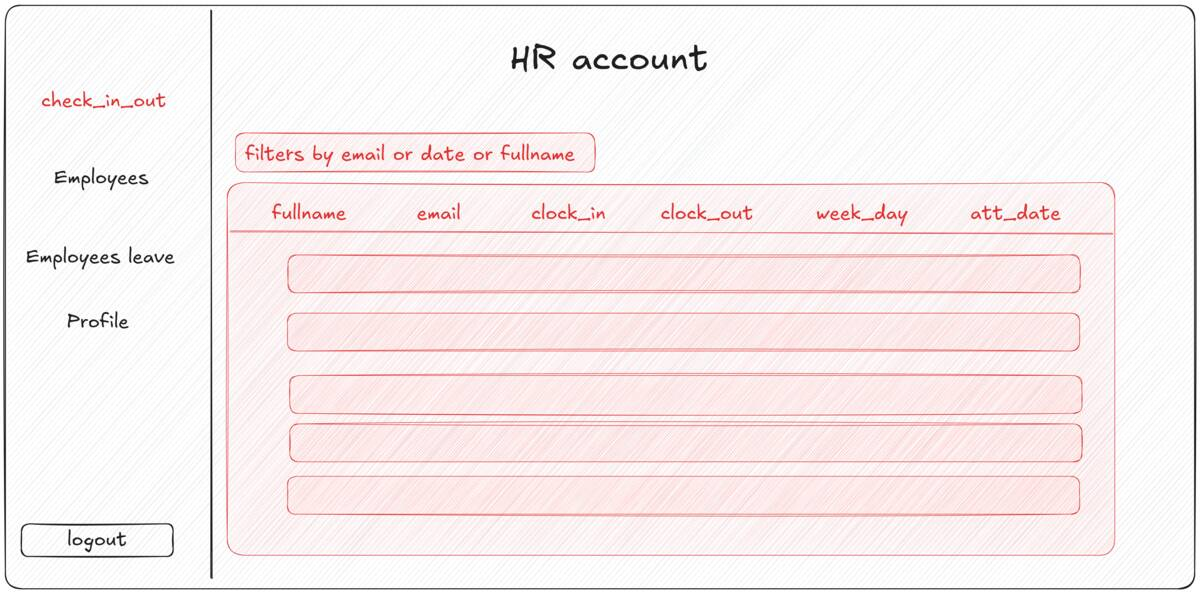
\includegraphics[width=0.92\textwidth,height=0.48\textheight,keepaspectratio]{assets/rh/checkinout-page-design-mockup.jpg}
}{%
    \fbox{\parbox{0.9\textwidth}{
    \centering
    \vspace{1.6cm}
    \textit{Missing file: assets/rh/checkinout-page-design-mockup.jpg}\\
    \textit{Insert Check-In/Out page design mockup.}
    \vspace{1.6cm}
    }}
}
\caption{Check-In/Out Page Design Mockup}
\label{fig:hr-checkinout-design-mockup}
\end{figure}

\subsection{Employee Leave page design mockup}
The Employee Leave page mockup explains attendance anomalies by showing leave periods and reasons in a readable, filterable layout linked to attendance investigations.

\begin{figure}[H]
\centering
\IfFileExists{assets/rh/employee-leave-page-design-mockup.jpg}{%
    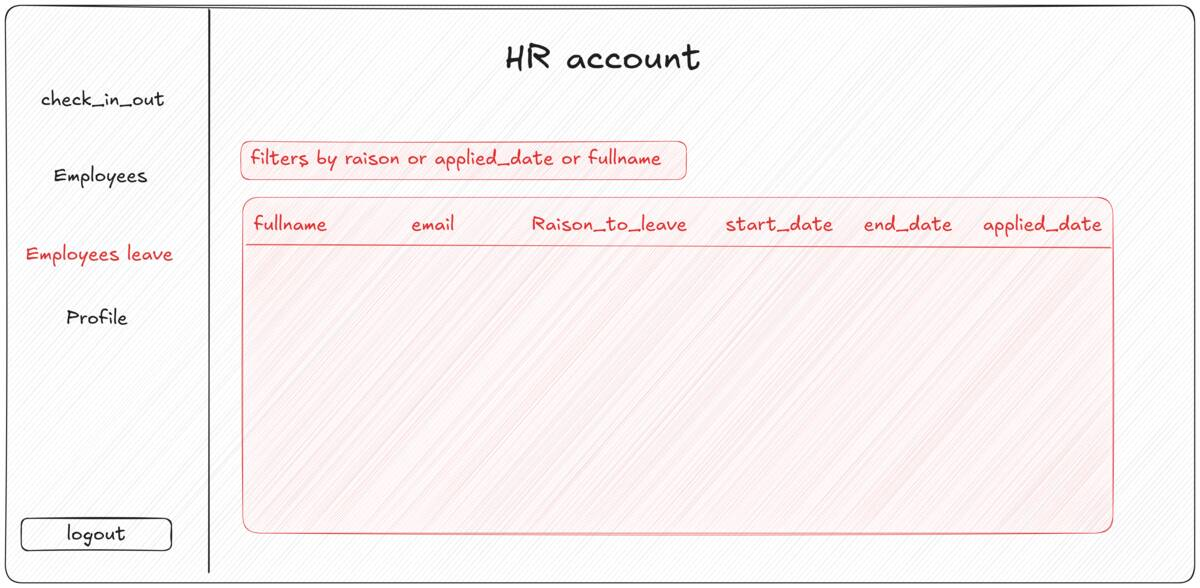
\includegraphics[width=0.92\textwidth,height=0.48\textheight,keepaspectratio]{assets/rh/employee-leave-page-design-mockup.jpg}
}{%
    \fbox{\parbox{0.9\textwidth}{
    \centering
    \vspace{1.6cm}
    \textit{Missing file: assets/rh/employee-leave-page-design-mockup.jpg}\\
    \textit{Insert Employee Leave page design mockup.}
    \vspace{1.6cm}
    }}
}
\caption{Employee Leave Page Design Mockup}
\label{fig:hr-leave-design-mockup}
\end{figure}

\section{Conception}
\subsection{HR use case diagram}
The HR use case model defines the main HR interactions: consult employees, analyze attendance check-in/out records, inspect leave reasons, and navigate between related records.

\begin{figure}[H]
\centering
\IfFileExists{diagrams/ch6-hr-use-case.jpg}{%
    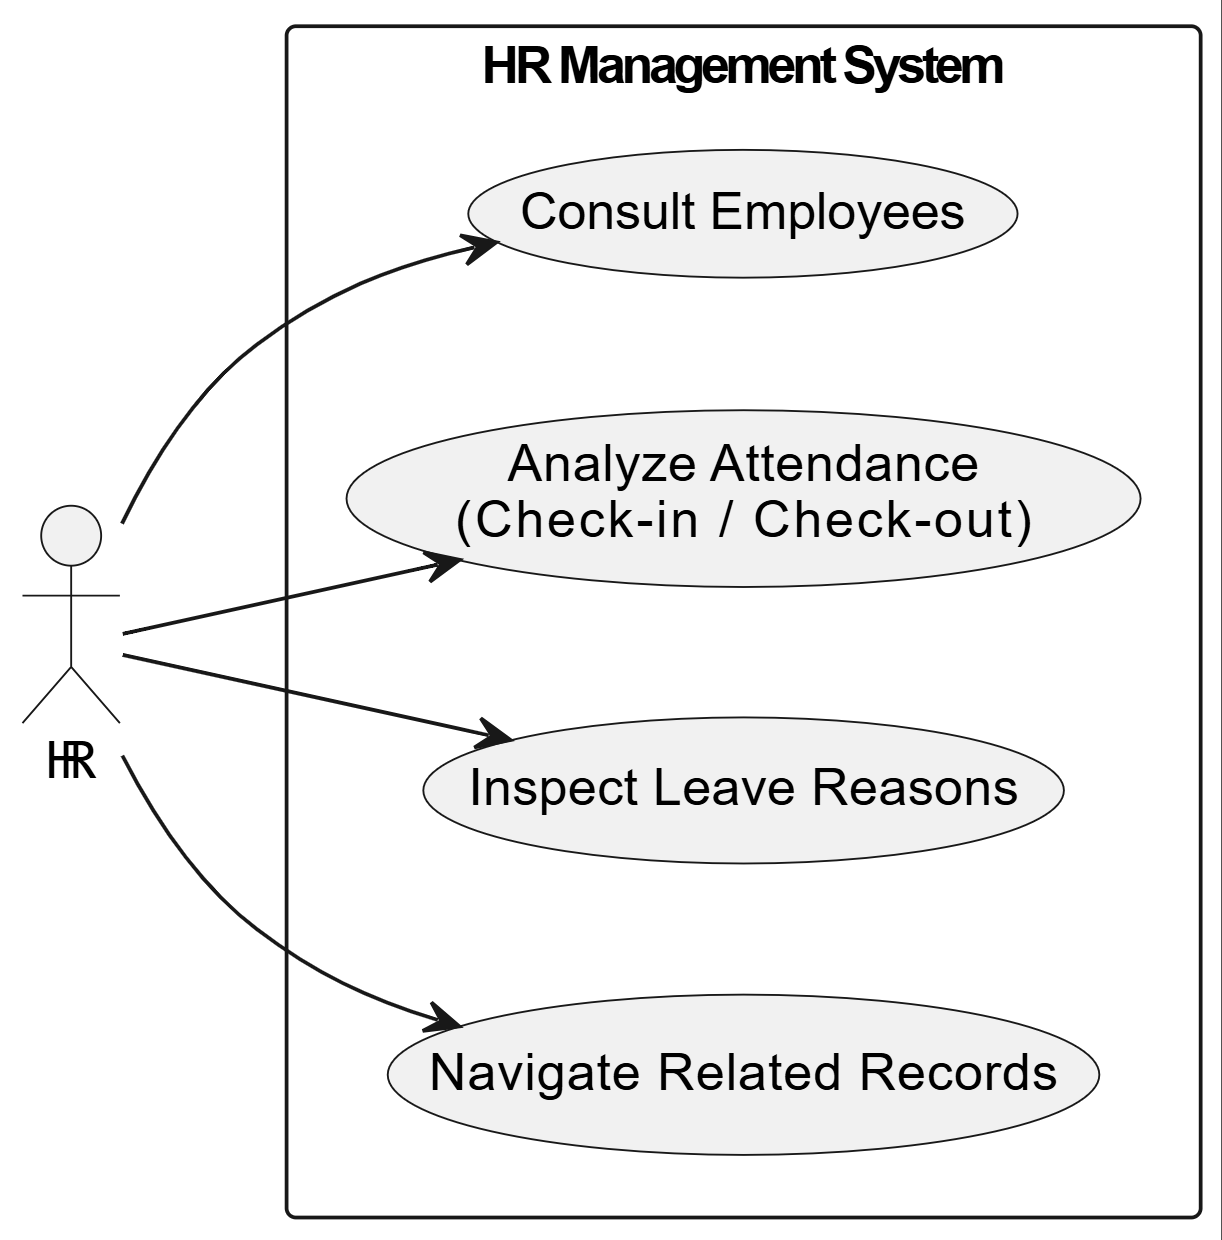
\includegraphics[width=0.92\textwidth,height=0.52\textheight,keepaspectratio]{diagrams/ch6-hr-use-case.jpg}
}{%
    \fbox{\parbox{0.9\textwidth}{
    \centering
    \vspace{1.6cm}
    \textit{Missing file: diagrams/ch6-hr-use-case.jpg}\\
    \textit{Insert HR Employee Attendance and Leave Monitoring use case diagram.}
    \vspace{1.6cm}
    }}
}
\caption{HR Employee Attendance and Leave Monitoring Use Case Diagram}
\label{fig:hr-use-case}
\end{figure}
Figure~\ref{fig:hr-use-case} summarizes the HR workflow across employee consultation, attendance tracking, and leave analysis.

\section{Sprint Realization}
\subsection{Implementation outcomes}
\begin{itemize}[noitemsep]
    \item Implemented Employees page with filters (name, email, department) and department donut chart.
    \item Implemented Check-In/Out page with attendance events and date-based filters.
    \item Implemented Employee Leave page with leave reasons linked to attendance gaps.
    \item Implemented redirect behavior from Check-In/Out rows to a pre-filtered Employee Leave view.
    \item Integrated pagination, filtering, TanStack Table, and TanStack Query caching across HR tables.
\end{itemize}

\subsection{Employees page interface}
\begin{figure}[H]
\centering
\IfFileExists{assets/rh/employees-page.jpg}{%
    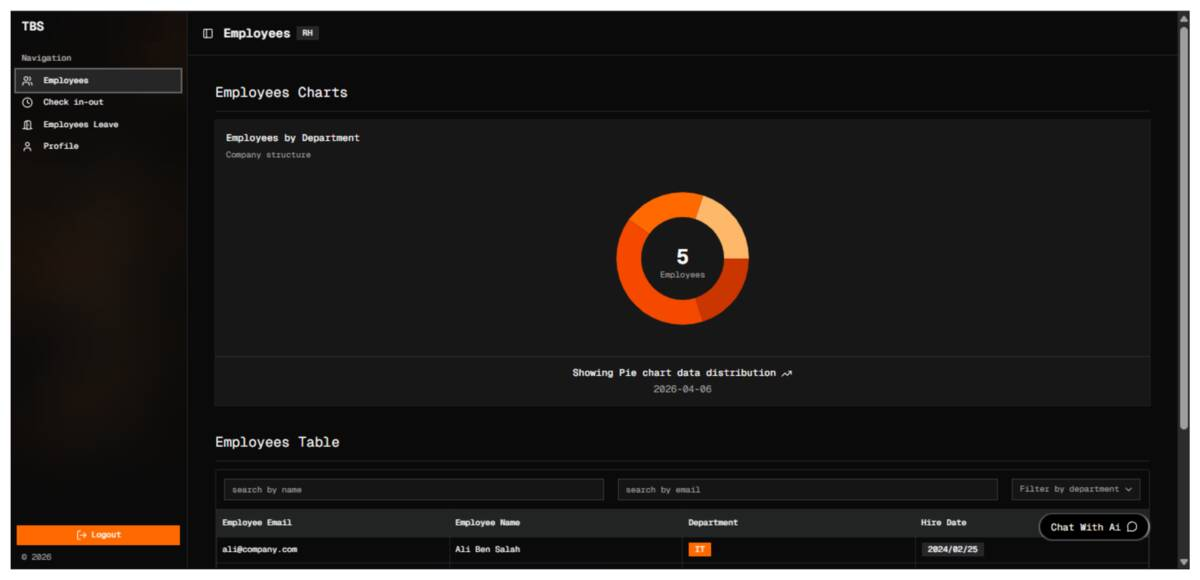
\includegraphics[width=0.92\textwidth,height=0.50\textheight,keepaspectratio]{assets/rh/employees-page.jpg}
}{%
    \fbox{\parbox{0.9\textwidth}{
    \centering
    \vspace{1.6cm}
    \textit{Missing file: assets/rh/employees-page.jpg}\\
    \textit{Insert HR Employees page (table + donut chart) screenshot.}
    \vspace{1.6cm}
    }}
}
\caption{HR Employees Page: Employee Directory and Department Donut Chart}
\label{fig:hr-employees-page}
\end{figure}
Figure~\ref{fig:hr-employees-page} shows the employee directory with filters and the donut chart used for department-level workforce distribution.

\subsection{Check-In/Out page interface}
\begin{figure}[H]
\centering
\IfFileExists{assets/rh/checkinout-page.jpg}{%
    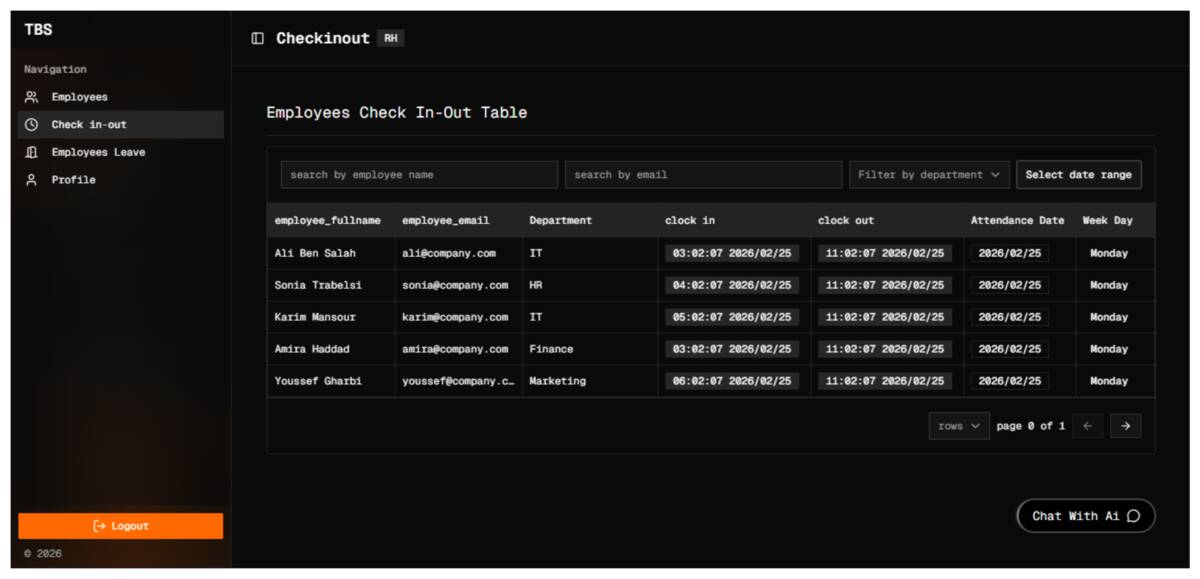
\includegraphics[width=0.92\textwidth,height=0.50\textheight,keepaspectratio]{assets/rh/checkinout-page.jpg}
}{%
    \fbox{\parbox{0.9\textwidth}{
    \centering
    \vspace{1.6cm}
    \textit{Missing file: assets/rh/checkinout-page.jpg}\\
    \textit{Insert HR Check-In/Out page screenshot.}
    \vspace{1.6cm}
    }}
}
\caption{HR Check-In/Out Page}
\label{fig:hr-checkinout-page}
\end{figure}
Figure~\ref{fig:hr-checkinout-page} illustrates attendance events with date filters for operational monitoring.

\subsection{Employee Leave page interface}
\begin{figure}[H]
\centering
\IfFileExists{assets/rh/employee-leave-page.jpg}{%
    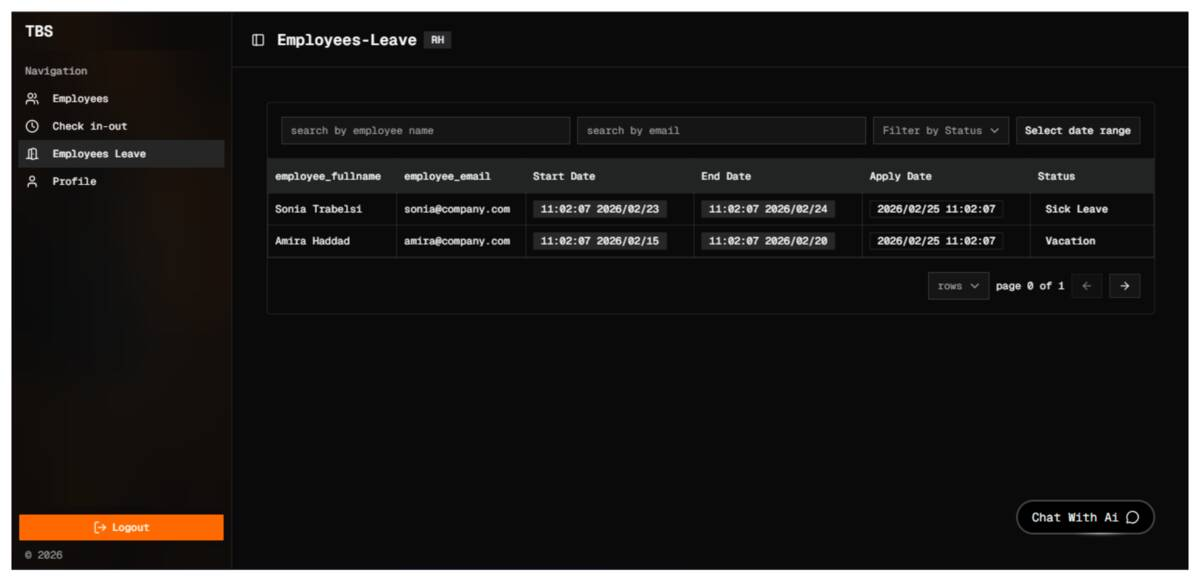
\includegraphics[width=0.92\textwidth,height=0.50\textheight,keepaspectratio]{assets/rh/employee-leave-page.jpg}
}{%
    \fbox{\parbox{0.9\textwidth}{
    \centering
    \vspace{1.6cm}
    \textit{Missing file: assets/rh/employee-leave-page.jpg}\\
    \textit{Insert HR Employee Leave page screenshot.}
    \vspace{1.6cm}
    }}
}
\caption{HR Employee Leave Page}
\label{fig:hr-leave-page}
\end{figure}
Figure~\ref{fig:hr-leave-page} presents leave details and reasons linked to missing attendance actions.

\section{Conclusion}
HR Employee Attendance and Leave Monitoring delivered a complete workflow for employee monitoring, attendance follow-up, and leave-based explanation of missing events. With scalable tables, smart navigation, and cached data access, these features support efficient HR operations on large datasets.
